% Created by tikzDevice version 0.12.3.1 on 2022-04-28 16:21:54
% !TEX encoding = UTF-8 Unicode
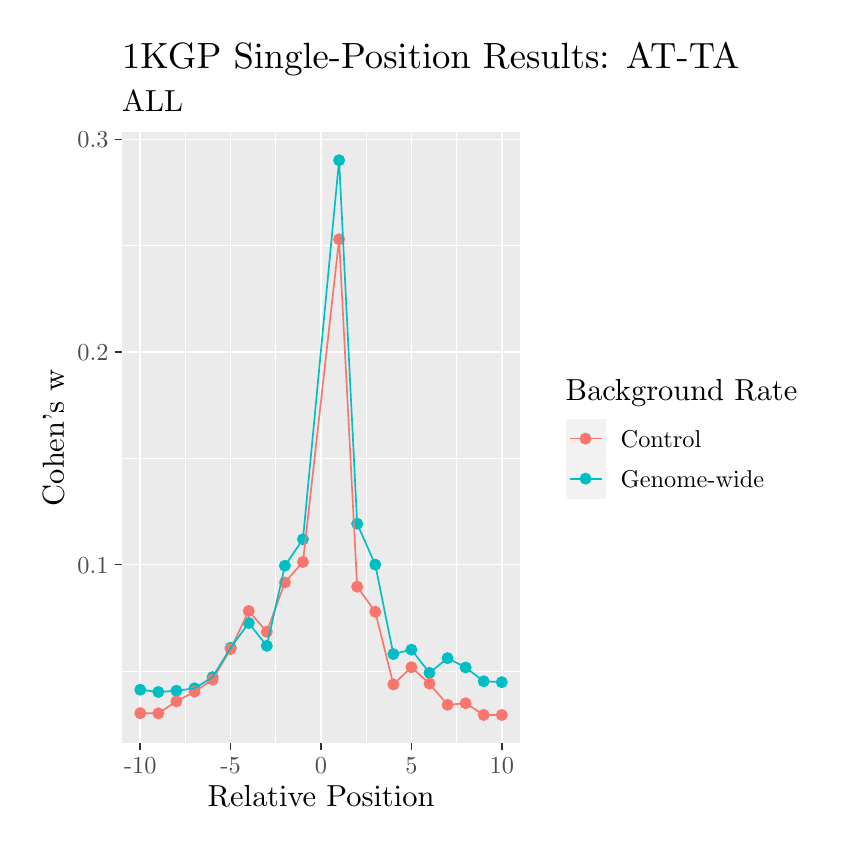
\begin{tikzpicture}[x=1pt,y=1pt]
\definecolor{fillColor}{RGB}{255,255,255}
\path[use as bounding box,fill=fillColor,fill opacity=0.00] (0,0) rectangle (289.08,289.08);
\begin{scope}
\path[clip] (  0.00,  0.00) rectangle (289.08,289.08);
\definecolor{drawColor}{RGB}{255,255,255}
\definecolor{fillColor}{RGB}{255,255,255}

\path[draw=drawColor,line width= 0.6pt,line join=round,line cap=round,fill=fillColor] (  0.00,  0.00) rectangle (289.08,289.08);
\end{scope}
\begin{scope}
\path[clip] ( 34.16, 30.69) rectangle (177.85,251.21);
\definecolor{fillColor}{gray}{0.92}

\path[fill=fillColor] ( 34.16, 30.69) rectangle (177.85,251.21);
\definecolor{drawColor}{RGB}{255,255,255}

\path[draw=drawColor,line width= 0.3pt,line join=round] ( 34.16, 56.63) --
	(177.85, 56.63);

\path[draw=drawColor,line width= 0.3pt,line join=round] ( 34.16,133.45) --
	(177.85,133.45);

\path[draw=drawColor,line width= 0.3pt,line join=round] ( 34.16,210.27) --
	(177.85,210.27);

\path[draw=drawColor,line width= 0.3pt,line join=round] ( 57.02, 30.69) --
	( 57.02,251.21);

\path[draw=drawColor,line width= 0.3pt,line join=round] ( 89.67, 30.69) --
	( 89.67,251.21);

\path[draw=drawColor,line width= 0.3pt,line join=round] (122.33, 30.69) --
	(122.33,251.21);

\path[draw=drawColor,line width= 0.3pt,line join=round] (154.99, 30.69) --
	(154.99,251.21);

\path[draw=drawColor,line width= 0.6pt,line join=round] ( 34.16, 95.04) --
	(177.85, 95.04);

\path[draw=drawColor,line width= 0.6pt,line join=round] ( 34.16,171.86) --
	(177.85,171.86);

\path[draw=drawColor,line width= 0.6pt,line join=round] ( 34.16,248.68) --
	(177.85,248.68);

\path[draw=drawColor,line width= 0.6pt,line join=round] ( 40.69, 30.69) --
	( 40.69,251.21);

\path[draw=drawColor,line width= 0.6pt,line join=round] ( 73.34, 30.69) --
	( 73.34,251.21);

\path[draw=drawColor,line width= 0.6pt,line join=round] (106.00, 30.69) --
	(106.00,251.21);

\path[draw=drawColor,line width= 0.6pt,line join=round] (138.66, 30.69) --
	(138.66,251.21);

\path[draw=drawColor,line width= 0.6pt,line join=round] (171.32, 30.69) --
	(171.32,251.21);
\definecolor{drawColor}{RGB}{0,191,196}
\definecolor{fillColor}{RGB}{0,191,196}

\path[draw=drawColor,line width= 0.4pt,line join=round,line cap=round,fill=fillColor] ( 40.69, 49.83) circle (  1.96);
\definecolor{drawColor}{RGB}{248,118,109}
\definecolor{fillColor}{RGB}{248,118,109}

\path[draw=drawColor,line width= 0.4pt,line join=round,line cap=round,fill=fillColor] ( 40.69, 41.38) circle (  1.96);
\definecolor{drawColor}{RGB}{0,191,196}
\definecolor{fillColor}{RGB}{0,191,196}

\path[draw=drawColor,line width= 0.4pt,line join=round,line cap=round,fill=fillColor] ( 47.22, 49.04) circle (  1.96);
\definecolor{drawColor}{RGB}{248,118,109}
\definecolor{fillColor}{RGB}{248,118,109}

\path[draw=drawColor,line width= 0.4pt,line join=round,line cap=round,fill=fillColor] ( 47.22, 41.31) circle (  1.96);
\definecolor{drawColor}{RGB}{0,191,196}
\definecolor{fillColor}{RGB}{0,191,196}

\path[draw=drawColor,line width= 0.4pt,line join=round,line cap=round,fill=fillColor] ( 53.75, 49.47) circle (  1.96);
\definecolor{drawColor}{RGB}{248,118,109}
\definecolor{fillColor}{RGB}{248,118,109}

\path[draw=drawColor,line width= 0.4pt,line join=round,line cap=round,fill=fillColor] ( 53.75, 45.63) circle (  1.96);
\definecolor{drawColor}{RGB}{0,191,196}
\definecolor{fillColor}{RGB}{0,191,196}

\path[draw=drawColor,line width= 0.4pt,line join=round,line cap=round,fill=fillColor] ( 60.28, 50.36) circle (  1.96);
\definecolor{drawColor}{RGB}{248,118,109}
\definecolor{fillColor}{RGB}{248,118,109}

\path[draw=drawColor,line width= 0.4pt,line join=round,line cap=round,fill=fillColor] ( 60.28, 49.17) circle (  1.96);
\definecolor{drawColor}{RGB}{0,191,196}
\definecolor{fillColor}{RGB}{0,191,196}

\path[draw=drawColor,line width= 0.4pt,line join=round,line cap=round,fill=fillColor] ( 66.81, 54.41) circle (  1.96);
\definecolor{drawColor}{RGB}{248,118,109}
\definecolor{fillColor}{RGB}{248,118,109}

\path[draw=drawColor,line width= 0.4pt,line join=round,line cap=round,fill=fillColor] ( 66.81, 53.52) circle (  1.96);
\definecolor{drawColor}{RGB}{0,191,196}
\definecolor{fillColor}{RGB}{0,191,196}

\path[draw=drawColor,line width= 0.4pt,line join=round,line cap=round,fill=fillColor] ( 73.34, 65.03) circle (  1.96);
\definecolor{drawColor}{RGB}{248,118,109}
\definecolor{fillColor}{RGB}{248,118,109}

\path[draw=drawColor,line width= 0.4pt,line join=round,line cap=round,fill=fillColor] ( 73.34, 64.54) circle (  1.96);
\definecolor{drawColor}{RGB}{0,191,196}
\definecolor{fillColor}{RGB}{0,191,196}

\path[draw=drawColor,line width= 0.4pt,line join=round,line cap=round,fill=fillColor] ( 79.88, 73.95) circle (  1.96);
\definecolor{drawColor}{RGB}{248,118,109}
\definecolor{fillColor}{RGB}{248,118,109}

\path[draw=drawColor,line width= 0.4pt,line join=round,line cap=round,fill=fillColor] ( 79.88, 78.29) circle (  1.96);
\definecolor{drawColor}{RGB}{0,191,196}
\definecolor{fillColor}{RGB}{0,191,196}

\path[draw=drawColor,line width= 0.4pt,line join=round,line cap=round,fill=fillColor] ( 86.41, 65.70) circle (  1.96);
\definecolor{drawColor}{RGB}{248,118,109}
\definecolor{fillColor}{RGB}{248,118,109}

\path[draw=drawColor,line width= 0.4pt,line join=round,line cap=round,fill=fillColor] ( 86.41, 70.79) circle (  1.96);
\definecolor{drawColor}{RGB}{0,191,196}
\definecolor{fillColor}{RGB}{0,191,196}

\path[draw=drawColor,line width= 0.4pt,line join=round,line cap=round,fill=fillColor] ( 92.94, 94.66) circle (  1.96);
\definecolor{drawColor}{RGB}{248,118,109}
\definecolor{fillColor}{RGB}{248,118,109}

\path[draw=drawColor,line width= 0.4pt,line join=round,line cap=round,fill=fillColor] ( 92.94, 88.60) circle (  1.96);
\definecolor{drawColor}{RGB}{0,191,196}
\definecolor{fillColor}{RGB}{0,191,196}

\path[draw=drawColor,line width= 0.4pt,line join=round,line cap=round,fill=fillColor] ( 99.47,104.21) circle (  1.96);
\definecolor{drawColor}{RGB}{248,118,109}
\definecolor{fillColor}{RGB}{248,118,109}

\path[draw=drawColor,line width= 0.4pt,line join=round,line cap=round,fill=fillColor] ( 99.47, 96.02) circle (  1.96);
\definecolor{drawColor}{RGB}{0,191,196}
\definecolor{fillColor}{RGB}{0,191,196}

\path[draw=drawColor,line width= 0.4pt,line join=round,line cap=round,fill=fillColor] (112.53,241.18) circle (  1.96);
\definecolor{drawColor}{RGB}{248,118,109}
\definecolor{fillColor}{RGB}{248,118,109}

\path[draw=drawColor,line width= 0.4pt,line join=round,line cap=round,fill=fillColor] (112.53,212.62) circle (  1.96);
\definecolor{drawColor}{RGB}{0,191,196}
\definecolor{fillColor}{RGB}{0,191,196}

\path[draw=drawColor,line width= 0.4pt,line join=round,line cap=round,fill=fillColor] (119.06,109.84) circle (  1.96);
\definecolor{drawColor}{RGB}{248,118,109}
\definecolor{fillColor}{RGB}{248,118,109}

\path[draw=drawColor,line width= 0.4pt,line join=round,line cap=round,fill=fillColor] (119.06, 87.08) circle (  1.96);
\definecolor{drawColor}{RGB}{0,191,196}
\definecolor{fillColor}{RGB}{0,191,196}

\path[draw=drawColor,line width= 0.4pt,line join=round,line cap=round,fill=fillColor] (125.60, 95.05) circle (  1.96);
\definecolor{drawColor}{RGB}{248,118,109}
\definecolor{fillColor}{RGB}{248,118,109}

\path[draw=drawColor,line width= 0.4pt,line join=round,line cap=round,fill=fillColor] (125.60, 78.02) circle (  1.96);
\definecolor{drawColor}{RGB}{0,191,196}
\definecolor{fillColor}{RGB}{0,191,196}

\path[draw=drawColor,line width= 0.4pt,line join=round,line cap=round,fill=fillColor] (132.13, 62.74) circle (  1.96);
\definecolor{drawColor}{RGB}{248,118,109}
\definecolor{fillColor}{RGB}{248,118,109}

\path[draw=drawColor,line width= 0.4pt,line join=round,line cap=round,fill=fillColor] (132.13, 51.76) circle (  1.96);
\definecolor{drawColor}{RGB}{0,191,196}
\definecolor{fillColor}{RGB}{0,191,196}

\path[draw=drawColor,line width= 0.4pt,line join=round,line cap=round,fill=fillColor] (138.66, 64.32) circle (  1.96);
\definecolor{drawColor}{RGB}{248,118,109}
\definecolor{fillColor}{RGB}{248,118,109}

\path[draw=drawColor,line width= 0.4pt,line join=round,line cap=round,fill=fillColor] (138.66, 57.98) circle (  1.96);
\definecolor{drawColor}{RGB}{0,191,196}
\definecolor{fillColor}{RGB}{0,191,196}

\path[draw=drawColor,line width= 0.4pt,line join=round,line cap=round,fill=fillColor] (145.19, 55.93) circle (  1.96);
\definecolor{drawColor}{RGB}{248,118,109}
\definecolor{fillColor}{RGB}{248,118,109}

\path[draw=drawColor,line width= 0.4pt,line join=round,line cap=round,fill=fillColor] (145.19, 52.06) circle (  1.96);
\definecolor{drawColor}{RGB}{0,191,196}
\definecolor{fillColor}{RGB}{0,191,196}

\path[draw=drawColor,line width= 0.4pt,line join=round,line cap=round,fill=fillColor] (151.72, 61.26) circle (  1.96);
\definecolor{drawColor}{RGB}{248,118,109}
\definecolor{fillColor}{RGB}{248,118,109}

\path[draw=drawColor,line width= 0.4pt,line join=round,line cap=round,fill=fillColor] (151.72, 44.40) circle (  1.96);
\definecolor{drawColor}{RGB}{0,191,196}
\definecolor{fillColor}{RGB}{0,191,196}

\path[draw=drawColor,line width= 0.4pt,line join=round,line cap=round,fill=fillColor] (158.25, 57.89) circle (  1.96);
\definecolor{drawColor}{RGB}{248,118,109}
\definecolor{fillColor}{RGB}{248,118,109}

\path[draw=drawColor,line width= 0.4pt,line join=round,line cap=round,fill=fillColor] (158.25, 44.96) circle (  1.96);
\definecolor{drawColor}{RGB}{0,191,196}
\definecolor{fillColor}{RGB}{0,191,196}

\path[draw=drawColor,line width= 0.4pt,line join=round,line cap=round,fill=fillColor] (164.78, 52.89) circle (  1.96);
\definecolor{drawColor}{RGB}{248,118,109}
\definecolor{fillColor}{RGB}{248,118,109}

\path[draw=drawColor,line width= 0.4pt,line join=round,line cap=round,fill=fillColor] (164.78, 40.74) circle (  1.96);
\definecolor{drawColor}{RGB}{0,191,196}
\definecolor{fillColor}{RGB}{0,191,196}

\path[draw=drawColor,line width= 0.4pt,line join=round,line cap=round,fill=fillColor] (171.32, 52.58) circle (  1.96);
\definecolor{drawColor}{RGB}{248,118,109}
\definecolor{fillColor}{RGB}{248,118,109}

\path[draw=drawColor,line width= 0.4pt,line join=round,line cap=round,fill=fillColor] (171.32, 40.71) circle (  1.96);

\path[draw=drawColor,line width= 0.6pt,line join=round] ( 40.69, 41.38) --
	( 47.22, 41.31) --
	( 53.75, 45.63) --
	( 60.28, 49.17) --
	( 66.81, 53.52) --
	( 73.34, 64.54) --
	( 79.88, 78.29) --
	( 86.41, 70.79) --
	( 92.94, 88.60) --
	( 99.47, 96.02) --
	(112.53,212.62) --
	(119.06, 87.08) --
	(125.60, 78.02) --
	(132.13, 51.76) --
	(138.66, 57.98) --
	(145.19, 52.06) --
	(151.72, 44.40) --
	(158.25, 44.96) --
	(164.78, 40.74) --
	(171.32, 40.71);
\definecolor{drawColor}{RGB}{0,191,196}

\path[draw=drawColor,line width= 0.6pt,line join=round] ( 40.69, 49.83) --
	( 47.22, 49.04) --
	( 53.75, 49.47) --
	( 60.28, 50.36) --
	( 66.81, 54.41) --
	( 73.34, 65.03) --
	( 79.88, 73.95) --
	( 86.41, 65.70) --
	( 92.94, 94.66) --
	( 99.47,104.21) --
	(112.53,241.18) --
	(119.06,109.84) --
	(125.60, 95.05) --
	(132.13, 62.74) --
	(138.66, 64.32) --
	(145.19, 55.93) --
	(151.72, 61.26) --
	(158.25, 57.89) --
	(164.78, 52.89) --
	(171.32, 52.58);
\end{scope}
\begin{scope}
\path[clip] (  0.00,  0.00) rectangle (289.08,289.08);
\definecolor{drawColor}{gray}{0.30}

\node[text=drawColor,anchor=base east,inner sep=0pt, outer sep=0pt, scale=  0.88] at ( 29.21, 92.01) {0.1};

\node[text=drawColor,anchor=base east,inner sep=0pt, outer sep=0pt, scale=  0.88] at ( 29.21,168.83) {0.2};

\node[text=drawColor,anchor=base east,inner sep=0pt, outer sep=0pt, scale=  0.88] at ( 29.21,245.65) {0.3};
\end{scope}
\begin{scope}
\path[clip] (  0.00,  0.00) rectangle (289.08,289.08);
\definecolor{drawColor}{gray}{0.20}

\path[draw=drawColor,line width= 0.6pt,line join=round] ( 31.41, 95.04) --
	( 34.16, 95.04);

\path[draw=drawColor,line width= 0.6pt,line join=round] ( 31.41,171.86) --
	( 34.16,171.86);

\path[draw=drawColor,line width= 0.6pt,line join=round] ( 31.41,248.68) --
	( 34.16,248.68);
\end{scope}
\begin{scope}
\path[clip] (  0.00,  0.00) rectangle (289.08,289.08);
\definecolor{drawColor}{gray}{0.20}

\path[draw=drawColor,line width= 0.6pt,line join=round] ( 40.69, 27.94) --
	( 40.69, 30.69);

\path[draw=drawColor,line width= 0.6pt,line join=round] ( 73.34, 27.94) --
	( 73.34, 30.69);

\path[draw=drawColor,line width= 0.6pt,line join=round] (106.00, 27.94) --
	(106.00, 30.69);

\path[draw=drawColor,line width= 0.6pt,line join=round] (138.66, 27.94) --
	(138.66, 30.69);

\path[draw=drawColor,line width= 0.6pt,line join=round] (171.32, 27.94) --
	(171.32, 30.69);
\end{scope}
\begin{scope}
\path[clip] (  0.00,  0.00) rectangle (289.08,289.08);
\definecolor{drawColor}{gray}{0.30}

\node[text=drawColor,anchor=base,inner sep=0pt, outer sep=0pt, scale=  0.88] at ( 40.69, 19.68) {-10};

\node[text=drawColor,anchor=base,inner sep=0pt, outer sep=0pt, scale=  0.88] at ( 73.34, 19.68) {-5};

\node[text=drawColor,anchor=base,inner sep=0pt, outer sep=0pt, scale=  0.88] at (106.00, 19.68) {0};

\node[text=drawColor,anchor=base,inner sep=0pt, outer sep=0pt, scale=  0.88] at (138.66, 19.68) {5};

\node[text=drawColor,anchor=base,inner sep=0pt, outer sep=0pt, scale=  0.88] at (171.32, 19.68) {10};
\end{scope}
\begin{scope}
\path[clip] (  0.00,  0.00) rectangle (289.08,289.08);
\definecolor{drawColor}{RGB}{0,0,0}

\node[text=drawColor,anchor=base,inner sep=0pt, outer sep=0pt, scale=  1.10] at (106.00,  7.64) {Relative Position};
\end{scope}
\begin{scope}
\path[clip] (  0.00,  0.00) rectangle (289.08,289.08);
\definecolor{drawColor}{RGB}{0,0,0}

\node[text=drawColor,rotate= 90.00,anchor=base,inner sep=0pt, outer sep=0pt, scale=  1.10] at ( 13.08,140.95) {Cohen's w};
\end{scope}
\begin{scope}
\path[clip] (  0.00,  0.00) rectangle (289.08,289.08);
\definecolor{fillColor}{RGB}{255,255,255}

\path[fill=fillColor] (188.85,113.39) rectangle (283.58,168.51);
\end{scope}
\begin{scope}
\path[clip] (  0.00,  0.00) rectangle (289.08,289.08);
\definecolor{drawColor}{RGB}{0,0,0}

\node[text=drawColor,anchor=base west,inner sep=0pt, outer sep=0pt, scale=  1.10] at (194.35,154.36) {Background Rate};
\end{scope}
\begin{scope}
\path[clip] (  0.00,  0.00) rectangle (289.08,289.08);
\definecolor{fillColor}{gray}{0.95}

\path[fill=fillColor] (194.35,133.34) rectangle (208.80,147.79);
\end{scope}
\begin{scope}
\path[clip] (  0.00,  0.00) rectangle (289.08,289.08);
\definecolor{drawColor}{RGB}{248,118,109}
\definecolor{fillColor}{RGB}{248,118,109}

\path[draw=drawColor,line width= 0.4pt,line join=round,line cap=round,fill=fillColor] (201.57,140.57) circle (  1.96);
\end{scope}
\begin{scope}
\path[clip] (  0.00,  0.00) rectangle (289.08,289.08);
\definecolor{drawColor}{RGB}{248,118,109}

\path[draw=drawColor,line width= 0.6pt,line join=round] (195.79,140.57) -- (207.36,140.57);
\end{scope}
\begin{scope}
\path[clip] (  0.00,  0.00) rectangle (289.08,289.08);
\definecolor{fillColor}{gray}{0.95}

\path[fill=fillColor] (194.35,118.89) rectangle (208.80,133.34);
\end{scope}
\begin{scope}
\path[clip] (  0.00,  0.00) rectangle (289.08,289.08);
\definecolor{drawColor}{RGB}{0,191,196}
\definecolor{fillColor}{RGB}{0,191,196}

\path[draw=drawColor,line width= 0.4pt,line join=round,line cap=round,fill=fillColor] (201.57,126.11) circle (  1.96);
\end{scope}
\begin{scope}
\path[clip] (  0.00,  0.00) rectangle (289.08,289.08);
\definecolor{drawColor}{RGB}{0,191,196}

\path[draw=drawColor,line width= 0.6pt,line join=round] (195.79,126.11) -- (207.36,126.11);
\end{scope}
\begin{scope}
\path[clip] (  0.00,  0.00) rectangle (289.08,289.08);
\definecolor{drawColor}{RGB}{0,0,0}

\node[text=drawColor,anchor=base west,inner sep=0pt, outer sep=0pt, scale=  0.88] at (214.30,137.54) {Control};
\end{scope}
\begin{scope}
\path[clip] (  0.00,  0.00) rectangle (289.08,289.08);
\definecolor{drawColor}{RGB}{0,0,0}

\node[text=drawColor,anchor=base west,inner sep=0pt, outer sep=0pt, scale=  0.88] at (214.30,123.08) {Genome-wide};
\end{scope}
\begin{scope}
\path[clip] (  0.00,  0.00) rectangle (289.08,289.08);
\definecolor{drawColor}{RGB}{0,0,0}

\node[text=drawColor,anchor=base west,inner sep=0pt, outer sep=0pt, scale=  1.10] at ( 34.16,258.85) {ALL};
\end{scope}
\begin{scope}
\path[clip] (  0.00,  0.00) rectangle (289.08,289.08);
\definecolor{drawColor}{RGB}{0,0,0}

\node[text=drawColor,anchor=base west,inner sep=0pt, outer sep=0pt, scale=  1.32] at ( 34.16,274.49) {1KGP Single-Position Results: AT-TA};
\end{scope}
\end{tikzpicture}
